\documentclass[12pt]{article}

\usepackage[T1]{fontenc}
\usepackage[polish]{babel}
\usepackage[utf8]{inputenc}
\usepackage{lmodern}
\selectlanguage{polish}

\usepackage{graphicx}
\usepackage{tabularx, booktabs}
\usepackage{fancyhdr} 
\usepackage{geometry}
\usepackage{hyperref}
\usepackage{listings}

\usepackage{subfigure}
\usepackage{longtable}
\usepackage{a4wide}

\usepackage{floatrow}

\geometry{left=15mm,right=25mm,%
bindingoffset=10mm, top=20mm, bottom=20mm}
 
\floatsetup[longtable]{LTcapwidth=table}


\renewcommand{\maketitle}{
\begin{titlepage}
\begin{table}[t]
\centering
\begin{tabular}[t]{lcr}
 
\includegraphics[width=70pt,height=70pt]{PW} & POLITECHNIKA WARSZAWSKA & 
\includegraphics[width=70pt,height=70pt]{MiNI}\\
& WYDZIAŁ MATEMATYKI & \\
& I NAUK INFORMACYJNYCH &
\end{tabular}
\end{table}
\vspace*{3cm}
  \begin{center}
    \LARGE
    \textbf {Raport}\\
   \vspace*{2 cm}
\begin{table}[!htp]
\begin{tabular}{p{4cm}p{10cm}}
\textit{Przedmiot:} &\textbf {Warsztaty z technik uczenia maszyn} \\
\\
\textit{Projekt:} &\textbf {Santander Customer Transaction Prediction} \\
\\
\textit{Autorzy:} &\textbf {Mateusz~Bieńkowski \newline
	Katarzyna~Gołębiewska \newline
	Filip~Grajek \newline
	Sebastian~Sudra \newline
	Łukasz~Sznajder \newline
	Nikodem~Wiśniewski \newline 
 } \\
\\
\end{tabular}
\end{table}

\vspace{5 cm}
  \center{\small Warszawa, dnia \today}
\end{center}
\end{titlepage}
}

\begin{document}
\maketitle

\newpage

\section{Opis projektu}

Projekt realizowany w ramach konkursu \textit{Santander Customer Transaction Prediction}\cite{santanderkaggle}. Celem projektu jest opracowanie jak klasyfikatora, który na podstawie dostępnych danych o konsumencie wskaże, czy dokona on transakcji czy też nie. 

\section{Opis danych}

Do dyspozycji uczestników konkursu organizator przygotował dwa zanonimizowane zbiory danych: \textit{train.csv} oraz \textit{test.csv}. Oba zbiory danych posiadają po 200 tysięcy wierszy. Każdy wiersz posiada identyfikator \textit{ID\_code} oraz 200 anonimowych cech (\textit{var0, var1 ... var199}). Zbiór \textit{train.csv} posiada dodatkowo kolumnę \textit{target} będącą etykietą, przyjmuje ona wartości $0$ lub $1$. Dane z pliku \textit{train.csv} służą do trenowania i wstępnej oceny jakości modelu. Plik \textit{test.csv} służy do oceny modelu przez organizatora konkursu, klasy dla tego zbioru nie są publicznie znane. Zgłoszeniem do konkursu jest plik zestawiający \textit{ID\_code} każdego rekordu z pliku \textit{test.csv} z jego przewidywaną klasą.


\subsection{Przetwarzanie i analiza danych}

Przetwarzanie i analiza danych są często uważane za najważniejsze narzędzia w osiąganiu ponadprzeciętnych wyników w zagadnieniach związanych ze sztuczną inteligencją. Przetwarzanie danych należy rozpocząć od sprawdzenia ich integralności. Przeszukanie wszystkich wierszy obu zbiorów nie wykazało żadnych brakujących pól. Kolejną ważną informacją jest liczba przykładów w obu klasach. Im bardziej nierównomierne są liczności zbiorów tym trudniej stworzyć model, który nie będzie się przeuczał w stronę wskazywania na liczniejszą klasę. Dla takich problemów nie można również korzystać z miary dokładności jaką jest procent prawidłowych klasyfikacji. W takich przypadkach należy użyć bardziej zaawansowanych metod porównywania modeli klasyfikacyjnych. Zbiór treningowy jest podzielony na 20098 (10.049\%) konsumentów, którzy dokonali transakcji oraz 179902 (89.951\%) konsumentów, którzy nie dokonali transakcji (rysunek \ref{classescount}). Dla zbioru testowego nie jesteśmy w stanie określić stosunku obu klas ze względu na brak etykiet. 
\begin{figure}[H]
\centering 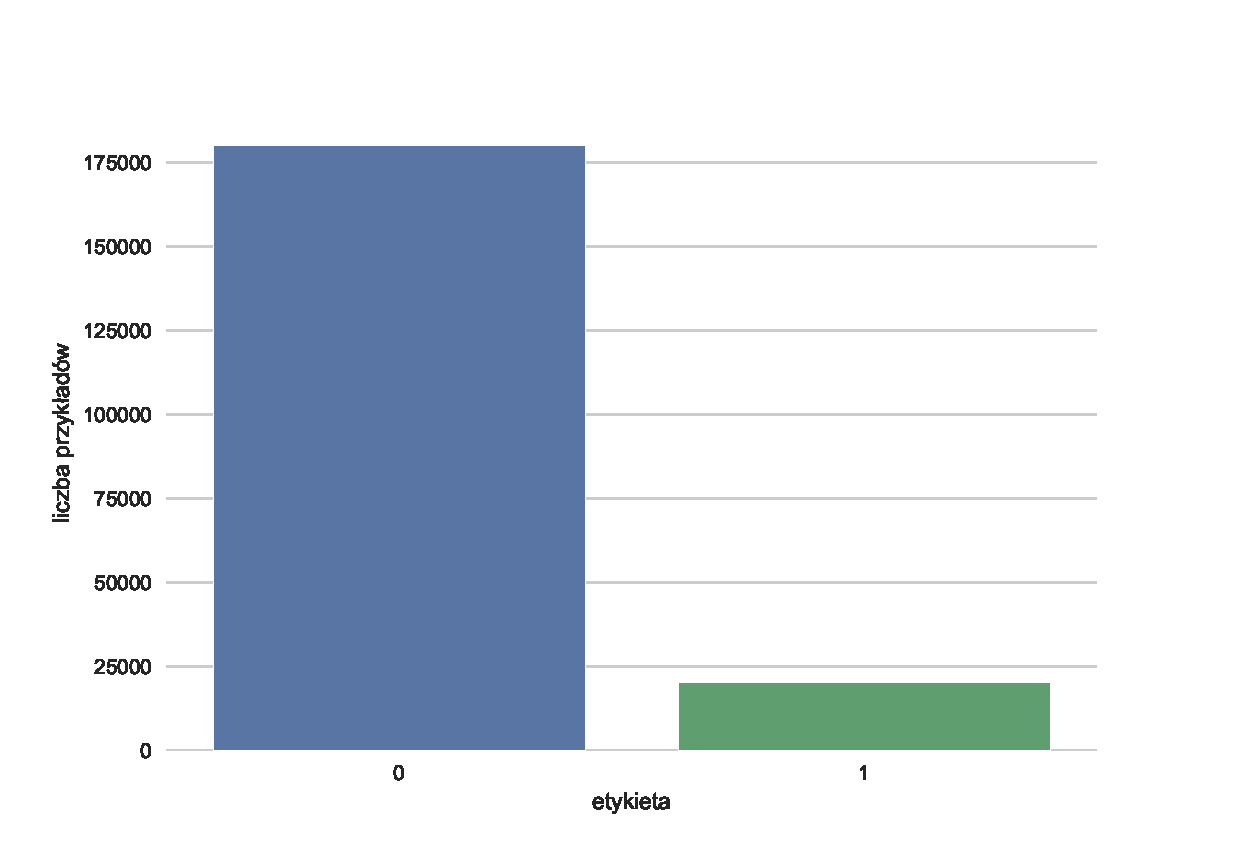
\includegraphics[scale=0.7]{classes.eps}
\caption{Liczba przykładów w każdej z klas}
\label{classescount}
\end{figure}
Jak widać klasy mocno różnią się licznością co negatywnie wpływa na poziom trudności całego zagadnienia.

\subsubsection{EDA (Exploratory Data Analysis)}

Eksploracyjne badanie danych jest podstawowym narzędziem w analizie danych pozwalającym na szczegółowy opis, wizualizację oraz badanie danych bez konieczności zakładania hipotez co do tych danych. Jest to w głównej mierze metoda oparta o statystykę, a jej wyniki pozwalają na ukierunkowanie kolejnych badań na konkretne cechy posiadanych danych. W tablicy \ref{traindescribe} widzimy dane statystyczne opisujące każdą z cech (kolumny kolejno: nazwa cechy, średnia, odchylenie standardowe, minimum, kwantyl 25\%, mediana, kwantyl 75\%, maksimum).

\begin{longtable}{lrrrrrrr}
\toprule
 feature &       mean &        std &      min &        25\% &       50\% &        75\% &      max \\
\midrule
\endhead
\midrule
\multicolumn{8}{r}{{Continued on next page}} \\
\midrule
\caption{Opis cech zbioru treningowego}
\label{traindescribe}
\endfoot

\bottomrule
\endlastfoot
   var\_0 &  10.679914 &   3.040051 &   0.4084 &   8.453850 &  10.52475 &  12.758200 &  20.3150 \\
   var\_1 &  -1.627622 &   4.050044 & -15.0434 &  -4.740025 &  -1.60805 &   1.358625 &  10.3768 \\
   var\_2 &  10.715192 &   2.640894 &   2.1171 &   8.722475 &  10.58000 &  12.516700 &  19.3530 \\
   var\_3 &   6.796529 &   2.043319 &  -0.0402 &   5.254075 &   6.82500 &   8.324100 &  13.1883 \\
   var\_4 &  11.078333 &   1.623150 &   5.0748 &   9.883175 &  11.10825 &  12.261125 &  16.6714 \\
   var\_5 &  -5.065317 &   7.863267 & -32.5626 & -11.200350 &  -4.83315 &   0.924800 &  17.2516 \\
   var\_6 &   5.408949 &   0.866607 &   2.3473 &   4.767700 &   5.38510 &   6.003000 &   8.4477 \\
   var\_7 &  16.545850 &   3.418076 &   5.3497 &  13.943800 &  16.45680 &  19.102900 &  27.6918 \\
   var\_8 &   0.284162 &   3.332634 & -10.5055 &  -2.317800 &   0.39370 &   2.937900 &  10.1513 \\
   var\_9 &   7.567236 &   1.235070 &   3.9705 &   6.618800 &   7.62960 &   8.584425 &  11.1506 \\
  var\_10 &   0.394340 &   5.500793 & -20.7313 &  -3.594950 &   0.48730 &   4.382925 &  18.6702 \\
  var\_11 &  -3.245596 &   5.970253 & -26.0950 &  -7.510600 &  -3.28695 &   0.852825 &  17.1887 \\
  var\_12 &  14.023978 &   0.190059 &  13.4346 &  13.894000 &  14.02550 &  14.164200 &  14.6545 \\
  var\_13 &   8.530232 &   4.639536 &  -6.0111 &   5.072800 &   8.60425 &  12.274775 &  22.3315 \\
  var\_14 &   7.537606 &   2.247908 &   1.0133 &   5.781875 &   7.52030 &   9.270425 &  14.9377 \\
  var\_15 &  14.573126 &   0.411711 &  13.0769 &  14.262800 &  14.57410 &  14.874500 &  15.8633 \\
  var\_16 &   9.333264 &   2.557421 &   0.6351 &   7.452275 &   9.23205 &  11.055900 &  17.9506 \\
  var\_17 &  -5.696731 &   6.712612 & -33.3802 & -10.476225 &  -5.66635 &  -0.810775 &  19.0259 \\
  var\_18 &  15.244013 &   7.851370 & -10.6642 &   9.177950 &  15.19625 &  21.013325 &  41.7480 \\
  var\_19 &  12.438567 &   7.996694 & -12.4025 &   6.276475 &  12.45390 &  18.433300 &  35.1830 \\
  var\_20 &  13.290894 &   5.876254 &  -5.4322 &   8.627800 &  13.19680 &  17.879400 &  31.2859 \\
  var\_21 &  17.257883 &   8.196564 & -10.0890 &  11.551000 &  17.23425 &  23.089050 &  49.0443 \\
  var\_22 &   4.305430 &   2.847958 &  -5.3225 &   2.182400 &   4.27515 &   6.293200 &  14.5945 \\
  var\_23 &   3.019540 &   0.526893 &   1.2098 &   2.634100 &   3.00865 &   3.403800 &   4.8752 \\
  var\_24 &  10.584400 &   3.777245 &  -0.6784 &   7.613000 &  10.38035 &  13.479600 &  25.4460 \\
  var\_25 &  13.667496 &   0.285535 &  12.7200 &  13.456400 &  13.66250 &  13.863700 &  14.6546 \\
  var\_26 &  -4.055133 &   5.922210 & -24.2431 &  -8.321725 &  -4.19690 &  -0.090200 &  15.6751 \\
  var\_27 &  -1.137908 &   1.523714 &  -6.1668 &  -2.307900 &  -1.13210 &   0.015625 &   3.2431 \\
  var\_28 &   5.532980 &   0.783367 &   2.0896 &   4.992100 &   5.53485 &   6.093700 &   8.7874 \\
  var\_29 &   5.053874 &   2.615942 &  -4.7872 &   3.171700 &   4.95020 &   6.798925 &  13.1431 \\
  var\_30 &  -7.687740 &   7.965198 & -34.7984 & -13.766175 &  -7.41175 &  -1.443450 &  15.6515 \\
  var\_31 &  10.393046 &   2.159891 &   2.1406 &   8.870000 &  10.36565 &  11.885000 &  20.1719 \\
  var\_32 &  -0.512886 &   2.587830 &  -8.9861 &  -2.500875 &  -0.49765 &   1.469100 &   6.7871 \\
  var\_33 &  14.774147 &   4.322325 &   1.5085 &  11.456300 &  14.57600 &  18.097125 &  29.5466 \\
  var\_34 &  11.434250 &   0.541614 &   9.8169 &  11.032300 &  11.43520 &  11.844400 &  13.2878 \\
  var\_35 &   3.842499 &   5.179559 & -16.5136 &   0.116975 &   3.91775 &   7.487725 &  21.5289 \\
  var\_36 &   2.187230 &   3.119978 &  -8.0951 &  -0.007125 &   2.19800 &   4.460400 &  14.2456 \\
  var\_37 &   5.868899 &   2.249730 &  -1.1834 &   4.125475 &   5.90065 &   7.542400 &  11.8638 \\
  var\_38 &  10.642131 &   4.278903 &  -6.3371 &   7.591050 &  10.56270 &  13.598925 &  29.8235 \\
  var\_39 &   0.662956 &   4.068845 & -14.5457 &  -2.199500 &   0.67230 &   3.637825 &  15.3223 \\
  var\_40 &  -6.725505 &   8.279259 & -35.2117 & -12.831825 &  -6.61745 &  -0.880875 &  18.1056 \\
  var\_41 &   9.299858 &   5.938088 &  -8.5359 &   4.519575 &   9.16265 &  13.754800 &  26.1658 \\
  var\_42 &  11.222356 &   0.695991 &   8.8590 &  10.713200 &  11.24340 &  11.756900 &  13.4696 \\
  var\_43 &  11.569954 &   0.309599 &  10.6528 &  11.343800 &  11.56500 &  11.804600 &  12.5779 \\
  var\_44 &   8.948289 &   5.903073 &  -9.9396 &   5.313650 &   9.43720 &  13.087300 &  34.1961 \\
  var\_45 & -12.699667 &  21.404912 & -90.2525 & -28.730700 & -12.54720 &   3.150525 &  62.0844 \\
  var\_46 &  11.326488 &   2.860511 &   1.2062 &   9.248750 &  11.31075 &  13.318300 &  21.2939 \\
  var\_47 & -12.471737 &  10.579862 & -47.6862 & -20.654525 & -12.48240 &  -4.244525 &  20.6854 \\
  var\_48 &  14.704713 &  11.384332 & -23.9022 &   6.351975 &  14.55920 &  23.028650 &  54.2738 \\
  var\_49 &  16.682499 &   7.855762 &  -8.0707 &  10.653475 &  16.67240 &  22.549050 &  41.1530 \\
  var\_50 &  12.740986 &   0.691709 &  10.3855 &  12.269000 &  12.74560 &  13.234500 &  15.3172 \\
  var\_51 &  13.428912 &   8.187306 & -15.0462 &   7.267625 &  13.44440 &  19.385650 &  40.6890 \\
  var\_52 &  -2.528816 &   4.985532 & -24.7214 &  -6.065025 &  -2.50245 &   0.944350 &  17.0968 \\
  var\_53 &   6.008569 &   0.764753 &   3.3449 &   5.435600 &   6.02780 &   6.542900 &   8.2315 \\
  var\_54 &   1.137117 &   8.414241 & -26.7786 &  -5.147625 &   1.27405 &   7.401825 &  28.5724 \\
  var\_55 &  12.745852 &   5.690072 &  -3.7826 &   8.163900 &  12.59410 &  17.086625 &  29.0921 \\
  var\_56 &  16.629165 &   3.540174 &   2.7618 &  14.097875 &  16.64815 &  19.289700 &  29.0741 \\
  var\_57 &   6.272014 &   0.795026 &   3.4423 &   5.687500 &   6.26250 &   6.845000 &   9.1609 \\
  var\_58 &   3.177633 &   4.296686 & -12.6009 &   0.183500 &   3.17010 &   6.209700 &  20.4833 \\
  var\_59 &   8.931124 &   0.854798 &   6.1840 &   8.312400 &   8.90100 &   9.566525 &  11.9867 \\
  var\_60 &  12.155618 &   4.222389 &  -2.1006 &   8.912750 &  12.06435 &  15.116500 &  25.1955 \\
  var\_61 & -11.946744 &  11.622948 & -48.8027 & -20.901725 & -11.89200 &  -3.225450 &  27.1029 \\
  var\_62 &   0.874170 &   2.026238 &  -6.3289 &  -0.572400 &   0.79470 &   2.228200 &   7.7536 \\
  var\_63 &   0.661173 &   3.113089 & -10.5544 &  -1.588700 &   0.68170 &   3.020300 &  11.2317 \\
  var\_64 &   6.369157 &   1.485854 &   1.6117 &   5.293500 &   6.37770 &   7.490600 &  11.1537 \\
  var\_65 &   0.982891 &   3.786493 & -14.0888 &  -1.702800 &   1.02135 &   3.739200 &  15.7313 \\
  var\_66 &   5.794039 &   1.121366 &   1.3368 &   4.973800 &   5.78200 &   6.586200 &   9.7132 \\
  var\_67 &  11.943223 &   7.365115 & -19.5443 &   6.753200 &  11.92200 &  17.037650 &  39.3968 \\
  var\_68 &   5.018893 &   0.007186 &   4.9938 &   5.014000 &   5.01910 &   5.024100 &   5.0469 \\
  var\_69 &  -3.331515 &   3.955723 & -16.3094 &  -6.336625 &  -3.32550 &  -0.498875 &   8.5473 \\
  var\_70 &  24.446811 &  11.951742 & -17.0275 &  15.256625 &  24.44500 &  33.633150 &  64.4644 \\
  var\_71 &   0.669756 &   0.266696 &  -0.2240 &   0.472300 &   0.66840 &   0.864400 &   1.5719 \\
  var\_72 &   0.640553 &   3.944703 & -12.3834 &  -2.197100 &   0.64645 &   3.510700 &  14.1500 \\
  var\_73 &  19.610888 &   7.466303 &  -1.6658 &  14.097275 &  19.30975 &  25.207125 &  44.5361 \\
  var\_74 &  19.518846 &  14.112591 & -34.1015 &   9.595975 &  19.53665 &  29.620700 &  70.2720 \\
  var\_75 &  16.853732 &   6.055322 &  -1.2936 &  12.480975 &  16.84420 &  21.432225 &  36.1567 \\
  var\_76 &   6.050871 &   7.938351 & -21.6333 &   0.596300 &   6.29780 &  11.818800 &  34.4352 \\
  var\_77 &  19.066993 &   3.817292 &   7.4257 &  16.014700 &  18.96785 &  22.041100 &  30.9569 \\
  var\_78 &   5.349479 &   1.993792 &  -1.8183 &   3.817275 &   5.44005 &   6.867200 &  11.3507 \\
  var\_79 &  14.402136 &   1.309055 &  10.4454 &  13.375400 &  14.38885 &  15.383100 &  18.2256 \\
  var\_80 &   5.795044 &   7.436737 & -18.0422 &   0.694475 &   6.06175 &  11.449125 &  30.4769 \\
  var\_81 &  14.719024 &   2.299567 &   7.5865 &  13.214775 &  14.84450 &  16.340800 &  23.1324 \\
  var\_82 &  -3.471273 &   8.479255 & -30.0266 & -10.004950 &  -3.28445 &   3.101725 &  21.8934 \\
  var\_83 &   1.025817 &   8.297229 & -24.2201 &  -5.106400 &   1.06970 &   7.449900 &  27.7143 \\
  var\_84 &  -2.590209 &   6.225305 & -24.4398 &  -7.216125 &  -2.51795 &   1.986700 &  17.7424 \\
  var\_85 &  18.362721 &   3.908536 &   7.0230 &  15.338575 &  18.29645 &  21.358850 &  32.9011 \\
  var\_86 &   5.621058 &   7.751142 & -19.2722 &   0.407550 &   6.00670 &  11.158375 &  34.5637 \\
  var\_87 &  11.351483 &   5.661867 &  -8.4816 &   7.247175 &  11.28800 &  15.433225 &  33.3541 \\
  var\_88 &   8.702924 &   2.491460 &   1.3502 &   6.918775 &   8.61620 &  10.567025 &  17.4594 \\
  var\_89 &   3.725208 &   3.560554 &  -9.6014 &   1.140500 &   3.64255 &   6.146200 &  15.4816 \\
  var\_90 & -16.548147 &  13.152810 & -61.7180 & -26.665600 & -16.48260 &  -6.409375 &  27.2713 \\
  var\_91 &   6.987541 &   0.152641 &   6.5218 &   6.869900 &   6.98650 &   7.101400 &   7.4895 \\
  var\_92 &  12.739578 &   4.186252 &  -1.0185 &   9.670300 &  12.67350 &  15.840225 &  26.9976 \\
  var\_93 &  10.556740 &   0.543341 &   8.4916 &  10.195600 &  10.58220 &  10.944900 &  12.5343 \\
  var\_94 &  10.999162 &   2.768099 &   2.8190 &   8.828000 &  10.98385 &  13.089100 &  18.9750 \\
  var\_95 &  -0.084344 &   0.621125 &  -2.4324 &  -0.527400 &  -0.09860 &   0.329100 &   1.8040 \\
  var\_96 &  14.400433 &   8.525400 & -12.1584 &   7.796950 &  14.36990 &  20.819375 &  40.8806 \\
  var\_97 &  18.539645 &  12.642382 & -21.7400 &   8.919525 &  18.50215 &  28.158975 &  58.2879 \\
  var\_98 &   1.752012 &   0.715836 &  -0.6035 &   1.267675 &   1.76830 &   2.260900 &   4.5028 \\
  var\_99 &  -0.746296 &   1.862550 &  -7.2806 &  -2.106200 &  -0.77130 &   0.528500 &   5.0764 \\
 var\_100 &  -6.600518 &   9.181683 & -39.1791 & -13.198700 &  -6.40150 &   0.132100 &  25.1409 \\
 var\_101 &  13.413526 &   4.950537 &   0.0757 &   9.639800 &  13.38085 &  17.250225 &  28.4594 \\
 var\_102 &  22.294908 &   8.628179 &  -7.3829 &  16.047975 &  22.30685 &  28.682225 &  51.3265 \\
 var\_103 &   1.568393 &   0.185020 &   0.9793 &   1.428900 &   1.56600 &   1.705400 &   2.1887 \\
 var\_104 &  11.509834 &   1.970520 &   4.0846 &  10.097900 &  11.49795 &  12.902100 &  19.0206 \\
 var\_105 &   4.244744 &   0.855698 &   0.7153 &   3.639600 &   4.22450 &   4.822200 &   7.1692 \\
 var\_106 &   8.617657 &   1.894899 &   0.9424 &   7.282300 &   8.60515 &   9.928900 &  15.3074 \\
 var\_107 &  17.796266 &   7.604723 &  -5.8980 &  12.168075 &  17.57320 &  23.348600 &  46.3795 \\
 var\_108 &  14.224435 &   0.171091 &  13.7290 &  14.098900 &  14.22660 &  14.361800 &  14.7430 \\
 var\_109 &  18.458001 &   4.355031 &   5.7697 &  15.107175 &  18.28135 &  21.852900 &  32.0591 \\
 var\_110 &   5.513238 &   3.823253 &  -9.2398 &   2.817475 &   5.39430 &   8.104325 &  19.5193 \\
 var\_111 &   6.312603 &   1.082404 &   2.1942 &   5.510100 &   6.34010 &   7.080300 &   9.8002 \\
 var\_112 &   3.317843 &   1.591170 &  -2.0302 &   2.092675 &   3.40840 &   4.577400 &   8.4317 \\
 var\_113 &   8.136542 &   4.459077 &  -5.5139 &   4.803250 &   8.14855 &  11.596200 &  21.5421 \\
 var\_114 &   3.081191 &   0.985396 &  -0.0505 &   2.388775 &   3.08380 &   3.811900 &   6.5850 \\
 var\_115 &   2.213717 &   2.621851 &  -6.8586 &   0.399700 &   2.24985 &   4.121500 &  11.9504 \\
 var\_116 &   2.402570 &   1.650912 &  -3.1630 &   1.171875 &   2.45630 &   3.665100 &   8.1207 \\
 var\_117 &  16.102233 &  13.297662 & -31.8369 &   6.373500 &  15.94485 &  25.780825 &  64.8109 \\
 var\_118 &  -5.305132 &   8.799268 & -37.5277 & -11.587850 &  -5.18950 &   0.971800 &  25.2635 \\
 var\_119 &   3.032849 &   4.182796 &  -9.7742 &  -0.161975 &   3.02395 &   6.098400 &  15.6885 \\
 var\_120 &  24.521078 &  12.121016 & -18.6962 &  15.696275 &  24.35470 &  33.105275 &  74.0321 \\
 var\_121 &  11.310591 &   1.714416 &   6.3052 &   9.996400 &  11.23970 &  12.619425 &  17.3074 \\
 var\_122 &   1.192984 &   5.168479 & -15.1940 &  -2.565200 &   1.20070 &   5.091700 &  18.4714 \\
 var\_123 &   7.076254 &   6.147345 & -12.4059 &   2.817050 &   7.23430 &  11.734750 &  26.8749 \\
 var\_124 &   4.272740 &   2.736821 &  -7.0538 &   2.353600 &   4.30210 &   6.192200 &  14.9915 \\
 var\_125 &  12.489165 &   0.318100 &  11.4861 &  12.245400 &  12.48630 &  12.718100 &  13.6642 \\
 var\_126 &  13.202326 &   0.776056 &  11.2654 &  12.608400 &  13.16680 &  13.811700 &  15.5156 \\
 var\_127 &   0.851507 &   3.137684 &  -8.8769 &  -1.502325 &   0.92500 &   3.293000 &  10.5976 \\
 var\_128 &  -1.127952 &   3.238043 & -11.7559 &  -3.580725 &  -1.10175 &   1.351700 &   9.8096 \\
 var\_129 &  15.460314 &   4.136453 &   2.1863 &  12.514475 &  15.42680 &  18.480400 &  31.2036 \\
 var\_130 &  12.257151 &   0.832199 &   9.5283 &  11.619300 &  12.26465 &  12.876700 &  14.9895 \\
 var\_131 &   0.544674 &   0.456280 &  -0.9548 &   0.207800 &   0.55660 &   0.901000 &   2.1923 \\
 var\_132 &   7.799676 &   1.456486 &   2.8900 &   6.724375 &   7.80910 &   8.911425 &  12.4650 \\
 var\_133 &   6.813270 &   0.375603 &   5.3593 &   6.543500 &   6.80670 &   7.070800 &   8.3091 \\
 var\_134 &  -4.826053 &   6.166126 & -24.2546 &  -9.625700 &  -4.70425 &  -0.178800 &  12.7236 \\
 var\_135 &  -4.259472 &   7.617732 & -31.3808 &  -9.957100 &  -4.11190 &   1.125950 &  21.4128 \\
 var\_136 &  22.968602 &  10.382235 &  -9.9493 &  14.933900 &  22.94830 &  31.042425 &  54.5794 \\
 var\_137 &  17.613651 &   8.890516 &  -9.8510 &  10.656550 &  17.25725 &  24.426025 &  44.4376 \\
 var\_138 &   1.210792 &   4.551750 & -16.4684 &  -2.011825 &   1.21175 &   4.391225 &  18.8187 \\
 var\_139 &   7.760193 &   7.686433 & -21.2743 &   2.387575 &   8.06625 &  13.232525 &  36.0971 \\
 var\_140 &   3.423636 &   4.896325 & -15.4595 &  -0.121700 &   3.56470 &   7.078525 &  21.1219 \\
 var\_141 &   2.897596 &   6.715637 & -16.6937 &  -2.153725 &   2.97550 &   8.192425 &  23.9658 \\
 var\_142 &  11.983489 &   5.691936 &  -7.1080 &   7.900000 &  11.85590 &  16.073925 &  32.8911 \\
 var\_143 &  12.333698 &   2.934706 &   2.8068 &  10.311200 &  12.35635 &  14.461050 &  22.6916 \\
 var\_144 &   8.647632 &   0.922469 &   5.4443 &   7.968075 &   8.65185 &   9.315000 &  11.8101 \\
 var\_145 &   4.841328 &   3.899281 &  -8.2734 &   1.885875 &   4.90470 &   7.676925 &  16.0083 \\
 var\_146 &  10.341178 &   2.518883 &   0.4274 &   8.646900 &  10.39560 &  12.113225 &  20.4373 \\
 var\_147 &  -3.300779 &   7.413301 & -29.9840 &  -8.751450 &  -3.17870 &   2.028275 &  22.1494 \\
 var\_148 &   3.990726 &   0.199192 &   3.3205 &   3.853600 &   3.99600 &   4.131600 &   4.7528 \\
 var\_149 &   5.296237 &  10.385133 & -41.1683 &  -1.903200 &   5.28325 &  12.688225 &  48.4240 \\
 var\_150 &  16.817671 &   2.464157 &   9.2420 &  14.952200 &  16.73695 &  18.682500 &  25.4357 \\
 var\_151 &  10.141542 &   3.962426 &  -2.1915 &   7.064600 &  10.12790 &  13.057600 &  21.1245 \\
 var\_152 &   7.633199 &   3.005373 &  -2.8800 &   5.567900 &   7.67370 &   9.817300 &  18.3846 \\
 var\_153 &  16.727902 &   2.014200 &  11.0308 &  15.233000 &  16.64975 &  18.263900 &  24.0075 \\
 var\_154 &   6.974955 &   4.961678 &  -8.1966 &   3.339900 &   6.99405 &  10.766350 &  23.2428 \\
 var\_155 &  -2.074128 &   5.771261 & -21.8409 &  -6.266025 &  -2.06610 &   1.891750 &  16.8316 \\
 var\_156 &  13.209272 &   0.955140 &   9.9965 &  12.475100 &  13.18430 &  13.929300 &  16.4970 \\
 var\_157 &  -4.813552 &   5.570272 & -22.9904 &  -8.939950 &  -4.86840 &  -0.988575 &  11.9721 \\
 var\_158 &  17.914591 &   7.885579 &  -4.5544 &  12.109200 &  17.63045 &  23.875325 &  44.7795 \\
 var\_159 &  10.223282 &   4.122912 &  -4.6416 &   7.243525 &  10.21755 &  13.094525 &  25.1200 \\
 var\_160 &  24.259300 &  10.880263 &  -7.4522 &  15.696125 &  23.86450 &  32.622850 &  58.3942 \\
 var\_161 &   5.633293 &   0.217938 &   4.8526 &   5.470500 &   5.63350 &   5.792000 &   6.3099 \\
 var\_162 &   5.362896 &   1.419612 &   0.6231 &   4.326100 &   5.35970 &   6.371200 &  10.1344 \\
 var\_163 &  11.002170 &   5.262056 &  -6.5317 &   7.029600 &  10.78870 &  14.623900 &  27.5648 \\
 var\_164 &  -2.871906 &   5.457784 & -19.9977 &  -7.094025 &  -2.63780 &   1.323600 &  12.1193 \\
 var\_165 &  19.315753 &   5.024182 &   3.8167 &  15.744550 &  19.27080 &  23.024025 &  38.3322 \\
 var\_166 &   2.963335 &   0.369684 &   1.8512 &   2.699000 &   2.96020 &   3.241500 &   4.2204 \\
 var\_167 &  -4.151155 &   7.798020 & -35.9695 &  -9.643100 &  -4.01160 &   1.318725 &  21.2766 \\
 var\_168 &   4.937124 &   3.105986 &  -5.2502 &   2.703200 &   4.76160 &   7.020025 &  14.8861 \\
 var\_169 &   5.636008 &   0.369437 &   4.2588 &   5.374600 &   5.63430 &   5.905400 &   7.0890 \\
 var\_170 &  -0.004962 &   4.424621 & -14.5060 &  -3.258500 &   0.00280 &   3.096400 &  16.7319 \\
 var\_171 &  -0.831777 &   5.378008 & -22.4793 &  -4.720350 &  -0.80735 &   2.956800 &  17.9173 \\
 var\_172 &  19.817094 &   8.674171 & -11.4533 &  13.731775 &  19.74800 &  25.907725 &  53.5919 \\
 var\_173 &  -0.677967 &   5.966674 & -22.7487 &  -5.009525 &  -0.56975 &   3.619900 &  18.8554 \\
 var\_174 &  20.210677 &   7.136427 &  -2.9953 &  15.064600 &  20.20610 &  25.641225 &  43.5468 \\
 var\_175 &  11.640613 &   2.892167 &   3.2415 &   9.371600 &  11.67980 &  13.745500 &  20.8548 \\
 var\_176 &  -2.799585 &   7.513939 & -29.1165 &  -8.386500 &  -2.53845 &   2.704400 &  20.2452 \\
 var\_177 &  11.882933 &   2.628895 &   4.9521 &   9.808675 &  11.73725 &  13.931300 &  20.5965 \\
 var\_178 &  -1.014064 &   8.579810 & -29.2734 &  -7.395700 &  -0.94205 &   5.338750 &  29.8413 \\
 var\_179 &   2.591444 &   2.798956 &  -7.8561 &   0.625575 &   2.51230 &   4.391125 &  13.4487 \\
 var\_180 &  -2.741666 &   5.261243 & -22.0374 &  -6.673900 &  -2.68880 &   0.996200 &  12.7505 \\
 var\_181 &  10.085518 &   1.371862 &   5.4165 &   9.084700 &  10.03605 &  11.011300 &  14.3939 \\
 var\_182 &   0.719109 &   8.963434 & -26.0011 &  -6.064425 &   0.72020 &   7.499175 &  29.2487 \\
 var\_183 &   8.769088 &   4.474924 &  -4.8082 &   5.423100 &   8.60000 &  12.127425 &  23.7049 \\
 var\_184 &  12.756676 &   9.318280 & -18.4897 &   5.663300 &  12.52100 &  19.456150 &  44.3634 \\
 var\_185 &  -3.983261 &   4.725167 & -22.5833 &  -7.360000 &  -3.94695 &  -0.590650 &  12.9975 \\
 var\_186 &   8.970274 &   3.189759 &  -3.0223 &   6.715200 &   8.90215 &  11.193800 &  21.7392 \\
 var\_187 & -10.335043 &  11.574708 & -47.7536 & -19.205125 & -10.20975 &  -1.466000 &  22.7861 \\
 var\_188 &  15.377174 &   3.944604 &   4.4123 &  12.501550 &  15.23945 &  18.345225 &  29.3303 \\
 var\_189 &   0.746072 &   0.976348 &  -2.5543 &   0.014900 &   0.74260 &   1.482900 &   4.0341 \\
 var\_190 &   3.234440 &   4.559922 & -14.0933 &  -0.058825 &   3.20360 &   6.406200 &  18.4409 \\
 var\_191 &   7.438408 &   3.023272 &  -2.6917 &   5.157400 &   7.34775 &   9.512525 &  16.7165 \\
 var\_192 &   1.927839 &   1.478423 &  -3.8145 &   0.889775 &   1.90130 &   2.949500 &   8.4024 \\
 var\_193 &   3.331774 &   3.992030 & -11.7834 &   0.584600 &   3.39635 &   6.205800 &  18.2818 \\
 var\_194 &  17.993784 &   3.135162 &   8.6944 &  15.629800 &  17.95795 &  20.396525 &  27.9288 \\
 var\_195 &  -0.142088 &   1.429372 &  -5.2610 &  -1.170700 &  -0.17270 &   0.829600 &   4.2729 \\
 var\_196 &   2.303335 &   5.454369 & -14.2096 &  -1.946925 &   2.40890 &   6.556725 &  18.3215 \\
 var\_197 &   8.908158 &   0.921625 &   5.9606 &   8.252800 &   8.88820 &   9.593300 &  12.0004 \\
 var\_198 &  15.870720 &   3.010945 &   6.2993 &  13.829700 &  15.93405 &  18.064725 &  26.0791 \\
 var\_199 &  -3.326537 &  10.438015 & -38.8528 & -11.208475 &  -2.81955 &   4.836800 &  28.5007 \\
\end{longtable}

Patrząc na dane z tablicy \ref{traindescribe} widać że odchylenie standardowe dużej liczby cech jest znaczne, co jest dobrą właściwością dla danych używanych w uczeniu maszynowym. Kolejnym wnioskiem jest podobny zakres wartości danych każdej cechy. Wszystkie wartości ze zbioru treningowego mieszczą się w zakresie $[-91, 75]$, co jest zaskakująco małym zakresem dla tak dużej liczby cech. Średnie wartości poszczególnych atrybutów również są bardzo zróżnicowane i wynoszą od $-16.5$ do $24.5$.

\subsubsection{PCA (Principal Component Analysis)}



\section{Ocena modeli}

Sposób oceny modeli został narzucony przez organizatorów konkursu. Ze względu na nierównomierny podział klas, do oceny modeli wykorzystana jest miara AUC, którą można uzyskać poprzez policzenie pola pod krzywą ROC.


\section{Modele klasyczne}

\section{Modele niekonwencjonalne}

\section{Wyniki i podsumowanie}


\newpage

\section{Bibliografia}
\begin{thebibliography}{9}

\bibitem{santanderkaggle}
\url{https://www.kaggle.com/c/santander-customer-transaction-prediction}

\bibitem{exampple}
  John Example,
  \textit{Example title}.
  Exampler,
  1996.

\end{thebibliography}

\end{document}